\documentclass[a4paper, twocolumn]{article}
\usepackage[pdftex, hidelinks,
            pdftitle={Report},
            pdfauthor={Erik S. Vasconcelos Jansson},
            pdfsubject={Report},
            pdfkeywords={report}]{hyperref}

\usepackage{bm}
\usepackage[T1]{fontenc}
\usepackage[utf8]{inputenc}
\usepackage{algpseudocode}
\usepackage{algorithm}
\usepackage{amsfonts}
\usepackage{booktabs}
\usepackage{amssymb}
\usepackage{courier}
\usepackage{booktabs}
\usepackage{graphicx}
\usepackage{listings}
\usepackage{mathtools}
\lstset{basicstyle=\footnotesize\ttfamily,
        breakatwhitespace = false,
        breaklines = true,
        keepspaces = true,
        language = C++,
        showspaces = false,
        showstringspaces = false,
        belowcaptionskip = \bigskipamount,
        framerule = 0.80pt,
        frame = tb,
        numbers = left,
        belowskip = \bigskipamount,
        escapeinside={<@}{@>}}

\title{Introduction to Machine Learning \\
       Individual Laboration Report --1--}
\author{{Erik Sven Vasconcelos Jansson} \\
        {\href{mailto:erija578@student.liu.se}
        {\texttt{erija578@student.liu.se}}} \\
        {Linköping University, \, Sweden}}

\begin{document}
    \pagenumbering{arabic}
    \maketitle % Titles...

    \section*{Assignment 1}

    Nobody likes \emph{e-mail spam}, therefore methods for autonomously \emph{predicting} if a given e-mail is probably \emph{spam} or \emph{not spam} is an important task. This is a classic example where \emph{machine learning} is useful; given a set of \emph{training data} and \emph{testing data}, can we predict what is \emph{spam} and \emph{not spam} in the \emph{testing set} (without knowing the answer) by deriving a \emph{hypothesis function} built from the \emph{training data}?

    By using \emph{k-nearest neighbor classification}, one can derive if an e-mail is spam or not by simply looking at \emph{similar e-mails/messages}, and picking the most likely solution by doing a \emph{``majority vote''}. First, a \emph{distance function} needs to be implemented, which is the \emph{cosine distance function} in Equation~\ref{eq:distance}, whose implementation can be found in Listing~\ref{lst:distance}, but with a optimized solution using only matrices.

    \begin{equation} \label{eq:distance}
        d(X,Y) = 1 - \frac{X^TY}{\sqrt{\sum_i{X_i^2}}\sqrt{\sum_i{Y_i^2}}}
    \end{equation}

    After defining the distance function $d(X,Y)$, one can find the \emph{e-mail/message distance} for each $Y_j$ in respect to each $X_i$. Where $X$ is the \emph{testing set} and $Y$ the \emph{training set}. Each row of the resulting matrix contains the relative distance between $X_i$ and $\forall Y_j$. Therefore, sorting each row $X_i$ and picking the first $K$ elements gives the $K$ \emph{closest messages} from the \emph{training set} in respect to each \emph{testing element}. By using this, the \emph{k-nearest neighbors} can be found, and the prediction of $\hat{Y}$ (spam, not spam) is done by using Equation~\ref{eq:knn}, where $K_i$ classify as being $C_i$.

    \begin{equation} \label{eq:knn}
        \hat{Y} = \underset{\forall C_i}{\mathrm{max}}\; p(C_i | \bm{x}),\; p(C_i | \bm{x}) \propto K_i \div K
    \end{equation}

    The \emph{k-nearest neighbor algorithm} is implemented in Listing~\ref{lst:knearest}, in the function \texttt{knearest(t,k,t')}. It works as previously described, where line \texttt{20} is calculating the \emph{distance matrix} and line \texttt{21} sorting each row, so that all $Y$ distances are relative to $X_i$. Thereafter, in line \texttt{26-27} the classification is found for the $K$-nearest neighbors of $X_i$. The \emph{mean} value is then taken, which is equivalent to $K_i \div K$ since only two classifications exist (spam and not spam), following a \emph{Cover et al.}~\cite{cover1967nearest} K-NN descriptions.

    Below follow \emph{confusion matrices} \& \emph{ROC curves}.

    \begin{table}[h]
    \begin{center}
    \begin{tabular}{r|c|c|}
        \multicolumn{1}{r}{\emph{k=5}}
        &\multicolumn{1}{c}{\textbf{false}}
        &\multicolumn{1}{c}{\textbf{true}} \\
        \cline{2-3}
        \textbf{false} & 778 & 349 \\
        \cline{2-3}
        \textbf{true} & 159 & 84 \\
        \cline{2-3}
    \end{tabular}
    \begin{tabular}{r|c|c|}
        \multicolumn{1}{r}{\emph{k=1}}
        &\multicolumn{1}{c}{\textbf{false}}
        &\multicolumn{1}{c}{\textbf{true}} \\
        \cline{2-3}
        \textbf{false} & 649 & 296 \\
        \cline{2-3}
        \textbf{true} & 288 & 137 \\
        \cline{2-3}
    \end{tabular}
    \end{center}
    \end{table}

    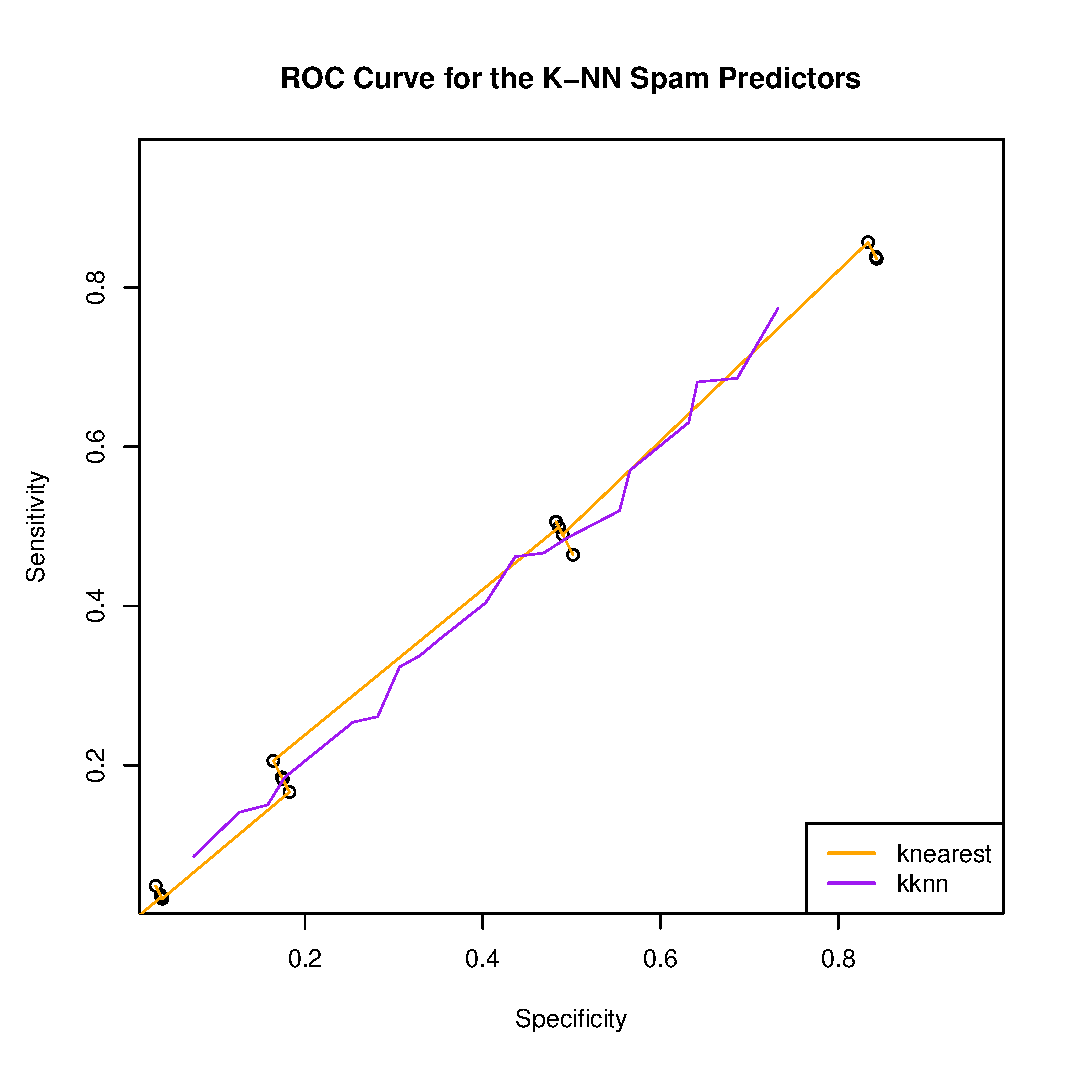
\includegraphics[width=0.5\textwidth]{share/spam.eps}

    \section*{Assignment 2}

    Knowing how to \emph{infer} what parameter $\theta$ most likely produced a already given data vector $\bm{x}$ is useful to gain more information about underlying processes. In this case, that is \emph{expected lifetime of machines}, which has been assumed to follow $p(\bm{x} | \theta) = \theta e^{-\theta x}$, where $\bm{x}$ are the \emph{expected lifetimes} of $n$ machines, which are independent and identically distributed. The P.D.F. $\theta e^{-\theta x}$ is from a \emph{exponential distribution}, as seen in \emph{Jonsson et al.}~\cite{jonsson1999ett}: $X \sim \mathrm{Exp}(\mu, \sigma^2)$...

    Estimation of the parameter $\theta$ can be done with \emph{MLE (Maximum Likelihood Estimation)}, which is usually done by using the \emph{log-likelihood} of $\theta$ for a given data vector $\bm{x}$. The formula for \emph{log-likelihood} is shown in Equation~\ref{eq:mle}, where the parameter $\theta$ can then be estimated with $\hat{\theta}_{mle}$ by selecting the most probable $\theta$ from a given set of thetas $\Theta, \theta_i \in \Theta$, by \emph{maximizing} the \emph{average log-likelihood}, as in Eq. 4. This is seen in e.g. \emph{Myung}~\cite{myung2003tutorial} and \emph{Wikipedia}.

    \begin{gather} \label{eq:mle}
        \mathcal{L}(\theta ; \bm{x}) = \mathrm{ln}\, p(\bm{x}|\theta) = \sum_{i=1}^{n}\mathrm{ln}\, p(x_i | \theta) \\
        \hat{\theta}_{mle} = \underset{\forall \theta}{\mathrm{max}}\, \mathcal{\hat{L}}(\theta ; \bm{x}),\; \mathcal{\hat{L}} = \frac{\mathrm{ln}\, p(\bm{x}|\theta)}{n}
    \end{gather}

    The actual implementation of these is found in Listing~\ref{lst:likelihood}, in the \emph{R} functions \texttt{lnlikelihood} and \texttt{distribution} (gives $\theta e^{-\theta x_i},\, \forall x_i \in \bm{x}$). For the MLE, lines \texttt{7-9} in Listing~\ref{lst:lifetime} calculate the \emph{average log-likelihood} and then picks the \emph{most probable} $\theta_i$. The MLE for the dataset shown in Listing~\ref{lst:machines} for when the \emph{entire dataset} is used, and when only $|\bm{x}| = 6$ is taken, is shown in the table to the right. As can be seen in the graph to the right, the $\hat{\theta}_{mle}$ for when $|\bm{x}| = 6$ will overshoot the value for when the actual full dataset is used, therefore, it is less reliable then when $|\bm{x}| = 48$, not a good estimator.

    If additional information is know about the distribution, in this case $p(\theta) = \lambda e^{-\lambda \theta}$ where $\lambda=10$, the \emph{MAP (Maximum a Posteriori)} estimation can be used instead. The implementation can be found in Listing~\ref{lst:likelihood}, in the \emph{R} function \texttt{polikelihood}. The MAP for the $\bm{x}$ dataset is shown in the table, and the graph for it is the green line to the right. Finally, taking random samples from the distribution with $\hat{\theta}_{mle}$ produces the histogram to the right.

    In conclusion, the parameter $\hat{\theta}_{mle}$ is a very good estimator for $\bm{x}$ given the Exp. distribution $p(\bm{x} | \theta)$.

    \newpage

    \begin{table}[h!]
    \begin{center}
    \begin{tabular}{lc}
        \toprule
            \textbf{Exp.\ Distribution} & \textbf{MLE/MAP} \\
        \midrule
            $p(\bm{x}|\theta), |\bm{x}|=48$ & 1.1 \\
            $p(\bm{x}|\theta), |\bm{x}|=6$ & 1.8 \\
            $p(\bm{x}|\theta)p(\theta), |\bm{x}|=48$ & 0.9 \\
        \bottomrule
    \end{tabular}
    \end{center}
    \end{table}

    \begin{figure}[h!]
        \centering
        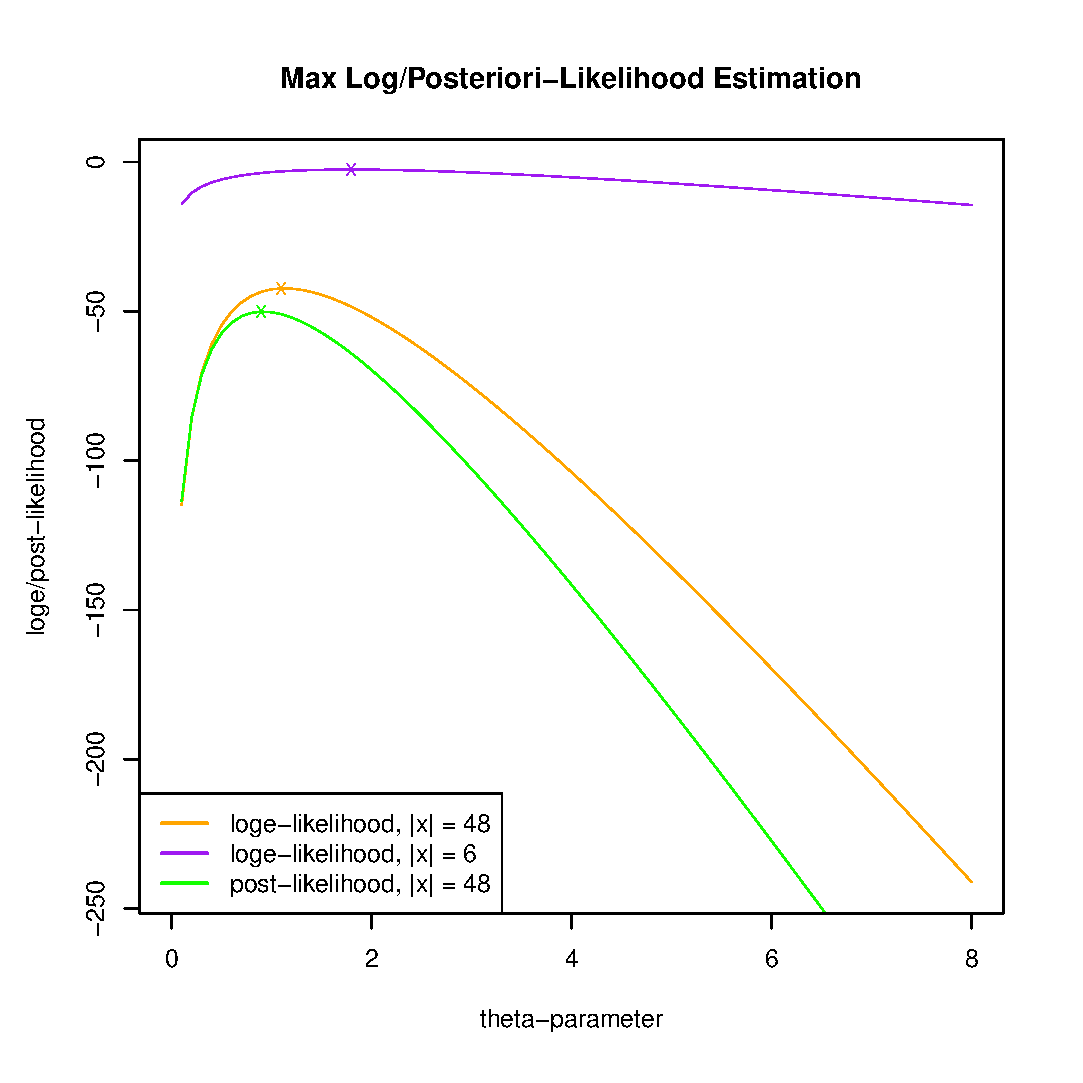
\includegraphics[width=0.5\textwidth]{share/machine.eps}
    \end{figure}

    \begin{figure}[h!]
        \centering
        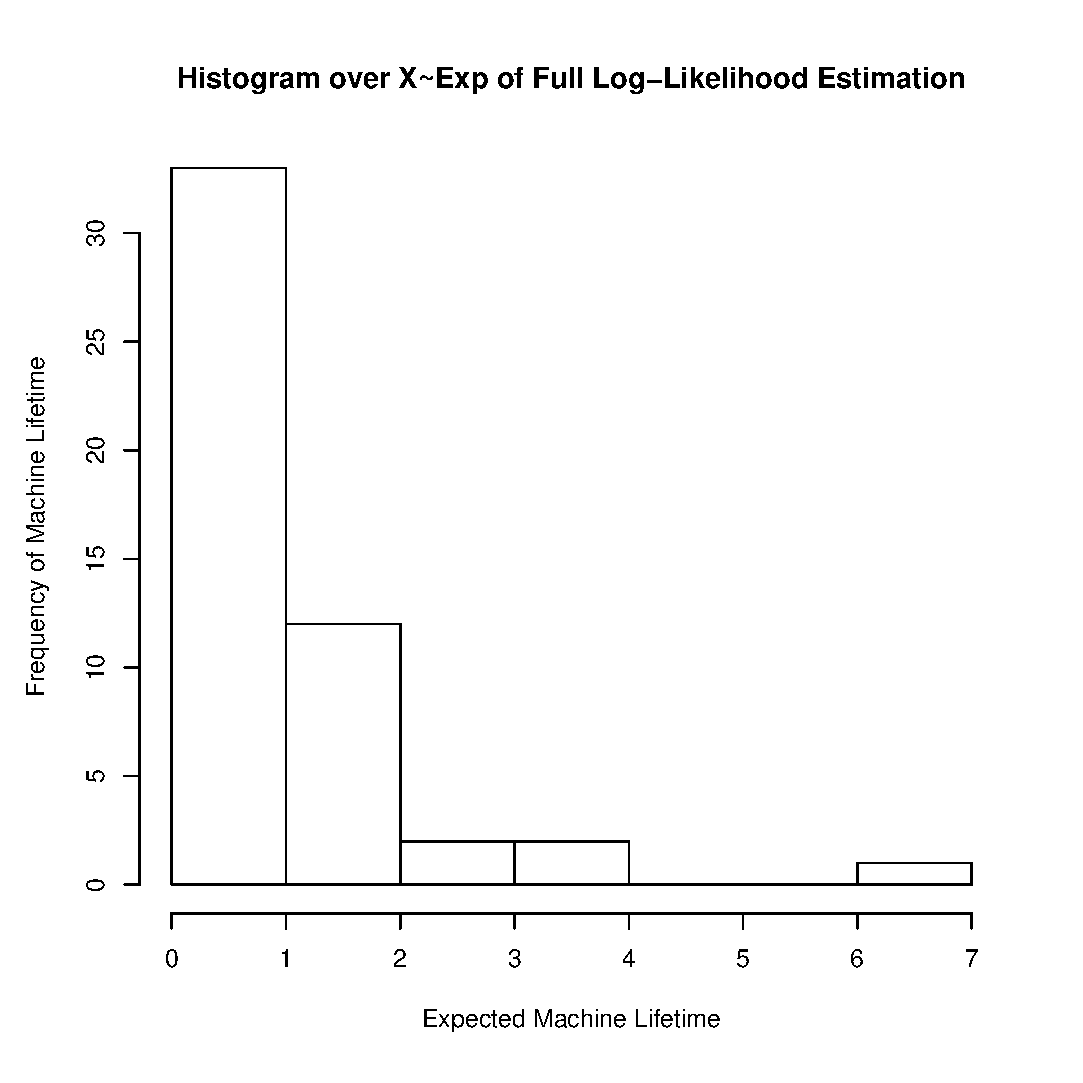
\includegraphics[width=0.5\textwidth]{share/histogram.eps}
    \end{figure}

    \clearpage \nocite{*}
    \bibliographystyle{alpha}
    \bibliography{report}

    \onecolumn \appendix
    \section*{Appendix}

    \lstinputlisting[caption={Spam Prediction Script},label={lst:spam}]{share/spam.r}
    \lstinputlisting[caption={K-Nearest Neighbor Algorithm Implementation},label={lst:knearest}]{share/knearest.r}
    \lstinputlisting[caption={Cosine Cost/Distance Formula},label={lst:distance}]{share/distance.r}
    \lstinputlisting[caption={Inference Script for Machine Lifetime},label={lst:lifetime}]{share/lifetime.r}
    \lstinputlisting[caption={Max Log- and Posteriori-Likelihood Estimation Formula},label={lst:likelihood}]{share/likelihood.r}
    \lstinputlisting[caption={The Given Machine Lifetime CSV Dataset (Excerpt)},label={lst:machines}, firstline=1, lastline=24]{share/machines.csv}

\end{document}
